
\section{Computation of CellML Models}\label{sec:computation_cellml_models}

In the following, we consider the computation of the subcellular model and other model that are given in CellML description.

The subcellular model is a system of DAEs that is solved at every node of the meshes in the discretized muscle.
For the fiber-based electrophysiology description, instances of the 0D subcellular model are computed on every node of every 1D fiber mesh. The 0D instances are coupled by the monodomain equation on every fiber. For the multidomain description, 0D model instances are solved at every node of the 3D muscle mesh for every compartment.

The subcellular model is provided as a CellML file and can be configured in the Python settings as described in \cref{sec:usage_cellml}.
The \code{CellMLAdapter} is the class in OpenDiHu that computes CellML model instances for all nodes of a given mesh. It computes the expression $G$ of the right hand side of the ODE system to obtain the vector of rates $\partial \bfy / \partial t = G(\bfy)$ and the expression $H$ for the algebraics $\bfh=H(\bfy)$. The new state vector $\bfy$ is computed from the previous vector by using the rates $\partial \bfy / \partial t$ according to a timestepping scheme.  In the solver tree, the timestepping solver class has to be the parent node of the \code{CellMLAdapter}.

CellML models can be obtained as C source files, which can be compiled to shared libraries, loaded and accessed by the solver program. This approach is used is both OpenCMISS and OpenDiHu.
The operation of computing multiple instances of a CellML model at once can be done more efficently than in the naive way of repeatedly executing the model function, as done in OpenCMISS. To exploit the structure of computing multiple model instances together, dedicated C code has to be generated from the CellML model at runtime for given numbers of model instances.
In the following, we describe our code generation functionality for this purpose.

\subsection{Data Flow for the Computation of CellML Models}

\begin{figure}%
  \centering%
  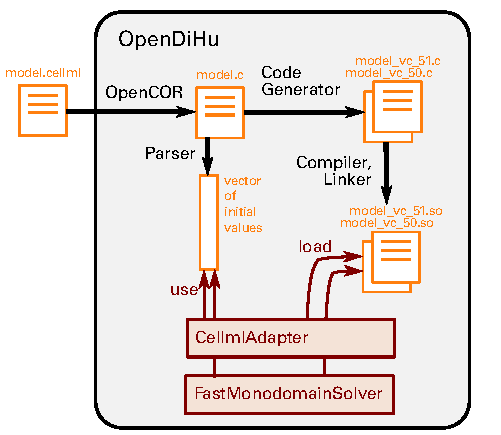
\includegraphics[width=0.7\textwidth]{images/implementation/cellml_scheme.pdf}%
  \caption{Processing of the given CellML model prior to solution. The CellML description is converted to C code using OpenCOR. The parser loads the C source code file and determines the contained initial values. Additionally, it parses the compute instructions into an internal syntax tree. The code generator produces optimizated C code that can solve as many instances of the model as needed on every process according to the global partitioning of the domain. The generated C code is compiled, linked to a shared library and accessed from the solver code.}
  \label{fig:cellml_scheme}%
\end{figure}%

\Cref{fig:cellml_scheme} shows the information flow for the CellML subsystem in OpenDiHu. On the left, a subcellular model is specified in CellML format in a file \code{model.cellml}. OpenDiHu uses the command line interface of OpenCOR to generate corresponding C code in the file \code{model.c}. A parser traverses the file and stores all instructions in an internal syntax tree data structure. The parser also determines the initial values for the state vector $\bfy$ from the code that initializes the variables.
Next, certain constants and algebraics in the compute instructions are replaced by parameter variables, as configured in the settings.

Then, a code generator outputs new C code that is optimized for a given number of CellML instances according to the number of nodes in the processes' subdomain within the global domain decomposition. 
This step is executed in parallel by different processes, but only once for every required number of model instances.

For example, if two fibers with 100 elements each are computed by $2 \times 2$ processes, the 101 nodes on each fiber are equally distributed to two different processes. As a result, each MPI rank has to compute either 51 or 50 CellML instances. Thus, the code generators on two of the ranks produce source code files for 51 and 50 model instances, named \code{model_vc_51.c} and \code{model_vc_50.c} in \cref{fig:cellml_scheme}, respectively. After generation, the source files are each compiled and linked to a shared library, resulting in the shared object files \code{model_vc_51.so} and \code{model_vc_50.so} in \cref{fig:cellml_scheme}.

The generation, compilation and linking steps are performed only by one process per source file.
If a source file or shared library with the required name already exists from a previous run, the steps are omitted.
In the example, only two processes generate and compile the code. All four processes synchronize after all shared libraries have been generated, before proceeding to execute the computations.

The generated shared libraries contain machine-code to compute the functions $G(\bfy)$ and $H(\bfy)$. They are loaded into the simulation program and executed by the \code{CellmlAdapter} class with the corresponding values, as indicated in \cref{fig:cellml_scheme}. Furthermore, the \code{CellmlAdapter} uses the previously inferred vector of initial values to initialize the state vector before the first timestep. Also the \code{FastMonodomainSolver} class presented in \cref{sec:improved_parallel_solver_for_fiber_based}, which efficiently solves the monodomain equation makes use of the code generator and the shared libraries to execute the subcellular model.

\subsection{Optimizations in the Generated Code}

The code generator can be configured to employ various types of optimizations in the generated code. These optimizations can be selected in the settings by the parameter \code{`optimizationType`}.

The naive way to solve multiple CellML model instances leads to storing the state vectors
in an Array-of-Struct (AoS) memory layout. The \say{struct} containing all components of the state vector for a single CellML model is stored at consecutive locations in memory and multiple structs for all computed instances are lined up next to each other. \Cref{fig:memory_layouts} shows the AoS layout in the top row for four model instances given by different colors. Each instance contains the three state variables $0,1$ and $2$. 

\begin{figure}%
  \centering%
  \begin{subfigure}[t]{0.6\textwidth}%
    \centering%
    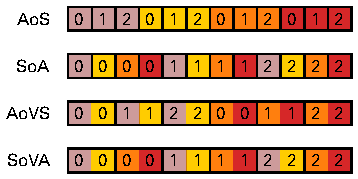
\includegraphics[width=\textwidth]{images/implementation/memory_layouts.pdf}
    \caption{Data in different memory layouts.}%
    \label{fig:memory_layouts}%
  \end{subfigure}\\[4mm]
  \begin{subfigure}[t]{0.7\textwidth}%
    \centering%
    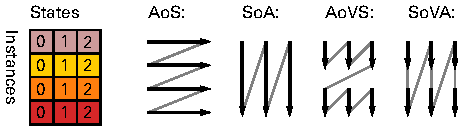
\includegraphics[width=\textwidth]{images/implementation/memory_layouts1.pdf}%
    \caption{Schemes how to construct the memory layouts. On the left, the entries are organized in a 2D field according to the state index and instance index. On the right, the traversal schemes for the different layouts are shown.}%
    \label{fig:memory_layouts1}%
  \end{subfigure}
  \caption{Different memory layouts for the CellML model: Array-of-Struct (AoS), Struct-of-Array (SoA), Array-of-Vectorized-Struct (AoVS), and Struct-of-Vectorized-Array (SoVA). The entries for four instances of the CellML model are shown by different colors and each instance dataset contains the three state variables 0,1 and 2.}%
  \label{fig:memory_layouts_both}%
\end{figure}%

The transposed memory layout is Struct-of-Array (SoA), where the same state components for all model instances are close in memory. In the example in the second row of \cref{fig:memory_layouts}, always four states of the same kind are stored contiguously. 
\Cref{fig:memory_layouts1} shows the construction schemes for the memory layouts. Comparing the scheme for SoA with AoS, it can be seen that the traversal in the 2D field of values is now vertical instead horizontal.

Such a vertical layout is a prerequisite for employing single-instruction-multiple-data (SIMD) parallelism. SIMD instructions perform the same calculations on multiple components of SIMD vectors simultaneously. In the visualization of SoA in \cref{fig:memory_layouts}, always four operands could be loaded simultaneously from memory to the vector registers in the CPU. Modern processors support the AVX2 instruction set with a SIMD lane width of $\mathcal{W}_T=4$ double values or the AVX-512 instruction set with $\mathcal{W}_T=8$ double values.

\begin{figure}
\centering
  \begin{subfigure}[t]{\textwidth}%
  \centering%
\begin{framed}
\begin{lstlisting}[basicstyle=\footnotesize\ttfamily,commentstyle=\color{gray},numbers=left]
  ALGEBRAIC[1] = ( - 0.100000*(STATES[0]+50.0000))/(exp(- (STATES[0]+50.0000)/10.0
  RATES[1] =  ALGEBRAIC[1]*(1.00000 - STATES[1]) -  ALGEBRAIC[5]*STATES[1];
  ...
\end{lstlisting}
\end{framed}
    \caption{Original C code for one CellML model instance generated by OpenCOR.}%
    \label{fig:cellml_codes_original}%
  \end{subfigure}\\[4mm]
  \begin{subfigure}[t]{\textwidth}%
  \centering%
\begin{framed}
\begin{lstlisting}[basicstyle=\footnotesize\ttfamily,commentstyle=\color{gray},numbers=left]
  #pragma omp for simd
  for (int i = 0; i < 1481; i++)
    algebraics[1481+i] = ( - 0.100000*(states[0+i]+50.0000))/(exp(- (states[0+i]+5
    
  #pragma omp for simd
  for (int i = 0; i < 1481; i++)
    rates[1481+i] =  algebraics[1481+i]*(1.00000 - states[1481+i]) -  algebraics[7
  ...
\end{lstlisting}
\end{framed}
    \caption{Generated code for optimization type \code{`simd`}.}%
    \label{fig:cellml_codes_simd}%
  \end{subfigure}\\[4mm]
  \begin{subfigure}[t]{\textwidth}%
  \centering%
\begin{framed}
\begin{lstlisting}[basicstyle=\footnotesize\ttfamily,commentstyle=\color{gray},numbers=left]
  // fill input vectors of states and parameters
  for (int stateNo = 0; stateNo < nStates; stateNo++)
    for (int i = 0; i < nVcVectors; i++)  // Vc vector no
      for (int k = 0; k < $\mathcal{W}_T$; k++)  // entry no in Vc vector 
        statesVc[i*nStates + stateNo][k] = states[stateNo*nInstances + i*$\mathcal{W}_T$+k]; $\label{alg:st_aovs}$
     // statesVc[stateNo*nVcVectors + i][k] = states[stateNo*nInstances + i*$\textcolor{gray}{\mathcal{W}_T}$+k]  $\label{alg:st_sova}$

  for (int i = 0; i < nVcVectors; i++)
  {
    algebraicsVc[i*nAlgebraics + 1] = ( - 0.100000*(statesVc[i*nStates + 0]+50.000 $\label{alg:b_aovs}$
  //algebraicsVc[371+i] = ( - 0.100000*(statesVc[0+i]+50.0000))/(exponential(- (st $\label{alg:b_sova}$
    ...
  }
\end{lstlisting}
\end{framed}
    \caption{Generated code for optimization type \code{`vc`}.}%
    \label{fig:cellml_codes_vc}%
  \end{subfigure}\\[4mm]
  \begin{subfigure}[t]{\textwidth}%
  \centering%
\begin{framed}
\begin{lstlisting}[basicstyle=\footnotesize\ttfamily,commentstyle=\color{gray},numbers=left]
  #pragma omp parallel for
  for (int i = 0; i < 1481; i++)
  {
    algebraics[1481+i] = ( - 0.100000*(states[0+i]+50.0000))/(exp(- (states[0+i]+5
    rates[1481+i] =  algebraics[1481+i]*(1.00000 - states[1481+i]) -  algebraics[7
    ...
  }
\end{lstlisting}
\end{framed}
    \caption{Generated code for optimization type \code{`openmp`}.}%
    \label{fig:cellml_codes_openmp}%
  \end{subfigure}
\caption{Output of the CellML code generator in OpenDiHu for 1481 model instances for different optimization types.  The model is the subcellular model of Hodgkin and Huxley and the code shows only two formulas of this model. Furthermore, the lines are truncated.}%
\label{fig:cellml_codes}%
\end{figure}

\Cref{fig:cellml_codes} demonstrates the code generation and presents different approaches to efficiently compute a CellML model for multiple instances. \Cref{fig:cellml_codes_original} shows the original code for a single model instance, which can be obtained from the CellML website or exported from a CellML model using OpenCOR. The listing shows the computation of the algebraic variable with index one and the rate with index one. The formulas typically use other states, algebraics and constant variables and consist of basic arithmetic such as additions, multiplications, potentiations to integer exponents and exponential functions. Some models, such as the subcellular model of Shorten et al. \cite{shorten2007mathematical} also involve piecewise definitions that include \say{inline if} branching operations.

Calling the code in \cref{fig:cellml_codes_original} for multiple model instances is associated with the AoS memory layout.
An improvement is the generated code with optimization type \code{`simd`} in \cref{fig:cellml_codes_simd}, which assumes the data to be organized in the SoA memory layout. The code is generated specifically to solved 1481 instances of the model. The array indexing for the \code{algebraics} and \code{rates} variables sums the constant offset according to the memory layout and the number of the model instance. For example, for the second algebraic (with former index 1) the offset is 1481 because so many memory locations are filled with values of the first algebraic (with former index 0).

Furthermore, every formula is enclosed in a loop over all 1481 instances of the model. The loops have OpenMP pragmas that instruct the compiler to use SIMD instructions for the loop body, if possible. Because of the consecutive storage, $\mathcal{W}_T$ loop iterations can be combined into a single computation using vector instructions. For the remainder iterations at the end of the loop, the compiler automatically adds different instructions with corresponding smaller SIMD vector lengths.

The approach of using OpenMP pragmas has the advantage that it is independent of the actual hardware capabilities and does not fix the SIMD vector size $\mathcal{W}_T$. If vectorization is disabled at compile-time, sequential CPU code is generated and the same valid solution is computed. A disadvantage is that the performance of the generated code depends on the vectorization ability of the compiler and its detection that the variables have the proper memory layout. For some constructs such as exponential functions or branching instructions, no vectorization is employed and the particular loop falls back to serial code. Such behavior is observed when inspecting the vectorization reports that are emitted by the compiler.

Thus, we implement another optimization type \code{`vc`} in the code generator that guarantees usage of vector instructions for all formulas. We use the C++ library \emph{Vc}, which provides a wrapper to hardware-specific vector instructions and abstracts the SIMD lane width \cite{vc2012,Kretz2015}. Using the data types of this library also allows to write hardware independent code and to achieve performance portability, like with the \code{`simd`} optimization type. 
As \emph{Vc} only supports vectorization up to the AVX2 instruction set, we also use the \code{std::experimental::simd} specification, which is currently considered by the International Organization for Standardization (ISO) and the International Electrotechnical Commission (IEC) for inclusion in the C++ standard library \cite{hoberock2016working}. Switching between these two libraries is transparent in the code and depends on whether the compiler has C++17 support.

Similar to the \code{`simd`} optimization type, the \code{`vc`} optimization type also uses a memory layout where consecutive memory entries correspond to different instances of the model and the traversal direction in \cref{fig:memory_layouts1} is vertical for at least $\mathcal{W}_T$ entries. \Cref{fig:memory_layouts_both} shows two such memory layouts for a SIMD vector length of $\mathcal{W}_T=2$: Array-of-Vectorized-Struct (AoVS) and Struct-of-Vectorized-Array (SoVA). Both are implemented in the code generator. 

The SoVA memory layout is very similar to SoA, the only difference is that in SoVA, entries are always accessed in multiples of the SIMD vector length $\mathcal{W}_T$. The advantage of SoVA is that the array indices are given by the sum of a constant offset with the loop index, whereas with the AoVS layout, a multiplication is required for every access.

AoVS resembles more the AoS layout. Its advantage over SoVA is that the complete state vector $\bfy$ for any model instance is located closer in memory. As the total computation iterates over model instances, the accessed memory is more coherent than for the same iteration scheme with the AoVS layout. This possibly leads to more cache hits, however for set-associative caches, the effect is reduced. Due to the complexity of today's cache architectures, only measurements can decide which of the two memory layouts lead to a faster execution. Our measurements show that the AoVS layout leads to \SI{2}{\percent} shorter runtimes than the SoVA memory layout and, thus, is the preferred choice.

%
%                     subdomains        user  total comp.         0D         1D  bidomain  duration_init     write       mem    n
% scenarioName nRanks                                                                                                            
% vc           18      [3, 2, 3]  186.429444   183.516278  45.524128  95.482744  2.693811       3.053507  1.707781  0.224 GB   18
% vc-aovs      18      [3, 2, 3]  178.800859   177.067879  44.365866  92.375215  2.323516       1.917626  1.673526  0.223 GB  198
% vc-sova      18      [3, 2, 3]  180.776722   179.158511  45.464952  93.226485  2.329576       1.810070  1.685208  0.223 GB  180
% ------------------------------------------------------------------------------------------------------------------------
% 

\Cref{fig:cellml_codes_vc} shows the resulting code using the AoVS memory layout. The commented out lines \ref{alg:st_sova} and \ref{alg:b_sova} show the corresponding code for the SoVA memory layout.
At the beginning of the generated program code, the given data in the \code{states} variable is copied to the \code{statesVc} variable in the new memory layout. Nested loops over all states, over the SIMD vectors and over the scalar values within the SIMD vector are used for this operation. For comparison, lines \ref{alg:st_aovs} and \ref{alg:st_sova} show the corresponding indexing of the \code{statesVc} variables for the AoVS and SoVA memory layouts, respectively.

For the computation of the model, we iterate over the number \code{nVcVectors} of SIMD vectors instead of the number of model instances as for \code{`simd`}. In the example with 1481 instances, we have \code{nVcVectors=$\lceil 1481/\mathcal{W}_T \rceil$=371} SIMD vectors for $\mathcal{W}_T=4$. 
Accordingly, the offsets for indexing the variables in the SoVA layout are smaller, e.g., in line \ref{alg:b_sova} the offset for indexing the \code{algebraicsVc} variables is now 371 instead of 1481 for the non-vectorized variable in the previously considered \code{`simd`} code. 
Comparing the statements for AoVS and SoVA in lines \ref{alg:b_aovs} and \ref{alg:b_sova}, it can be seen that the AoVS memory layout involves an additional multiplication during the indexing of the array.

In case of branching instructions in the CellML formulas, the Vc library provides an implementation of the \say{inline if} statement for SIMD vectors that checks the condition, potentially executes both branches and merges the components from the active branches into the resulting SIMD vector.

Profiling the execution of the \code{`vc`} code for different subcellular models shows that about half of the runtime is spent in evaluating the exponential function. Therefore, we use the following approximation:
\begin{align*}
  \textrm{exp}(x) \approx \textrm{exp}^\ast(x) = \left( 1 + \dfrac{x}{n}\right)^n.
\end{align*}
The series converges to the exact value for $n\to \infty$. We choose $n=1024$ and are able to compute the approximate value by only one addition and 11 multiplications using the following formula:
\begin{align*}
    \textrm{exp}^\ast(x) = \left( 1 + \dfrac{x}{1024}\right)^{2^{10}} = {{{\left( 1 + \dfrac{x}{1024}\right)^2}^2}^{\scriptsize\iddots}}^2.
\end{align*}
%
In the subcellular models of Hodgkin and Huxley \cite{Hodgkin1952} and Shorten et al. \cite{shorten2007mathematical}, the values for $x$ are bounded by $|x| < x_\text{max} = 12$, and we get a relative error of the approximation of $|(\textrm{exp}^\ast - \textrm{exp})(x_\text{max}) / \textrm{exp}(x_\text{max})| < 0.07.$
This approximation can be enabled or disabled in the code generation.

Another optimization is implemented for exponentiation $a^b$. In the considered CellML models, only integer exponents $b\in \mathbb{Z}$ occur. We add a recursive implementation of the power function that requires a logarithmic number of multiplications. 

The code generator with the \code{`vc`} optimization type is also used by the \code{FastMonodomain}\code{Solver} class described in \cref{sec:improved_parallel_solver_for_fiber_based}. The generated codes for the \code{FastMonodomainSolver} class additionally contain the Heun scheme to solve the model, integrate code for the stimulation of muscle fibers and  export certain algebraic values that were declared as parameters in the settings.

Another possiblity to improve the performance besides instruction-level parallelism is thread-level parallelism. The \code{`openmp`} optimization type generates code containing OpenMP pragmas that distribute the computations to multiple OpenMP threads with shared memory. \Cref{fig:cellml_codes_openmp} shows the generated code for this optimization type. A loop iterates over all model instances and the variables are stored in SoA memory layout. The loop iterations are independent of each other as they correspond to different instances of the CellML model. OpenMP distributes the workload to a predefined number of threads that can be specified by environment variables.

\subsection{Code Generation for GPUs}

Besides instruction-level and thread-level parallelism, which were discussed in the last section, accelerator hardware such as GPUs can be considered to reduce the runtime of solving a CellML model.
Our code generator features the \code{`gpu`} optimization type to generate code that is called on the CPU and then offloads the main computations to a GPU.

We use OpenMP 4.5 to instrument the generated code for device offloading. At the time of writing, only an experimental version of GCC 11 is fully capable of compiling this code. In our studies, the code is compiled for the \emph{nvptx} target which generates and compiles device-specific CUDA code using the NVIDIA parallel thread execution (PTX) instruction set architecture. We successfully run the computation on various NVIDIA GPUs, including a GeForce RTX 3080. However, the approach is device-agnostic and other accelerator hardware can also be used.

\Cref{fig:cellml_codes_gpu} shows an excerpt of the generated code. It resembles the code of the\break\code{`openmp`} optimization type, except that the OpenMP pragma in lines \ref{alg:pragma_line} and \ref{alg:pragma_line2} is different. The lines specify the variables to be mapped to and from the target device: The vectors of states and parameters as well as the current simulation time \code{t} are send to the GPU and, after computation, the rates and algebraics are transferred back to the CPU.

\begin{figure}
\centering
\begin{framed}
\begin{lstlisting}[basicstyle=\footnotesize\ttfamily,commentstyle=\color{gray},numbers=left]
  #pragma omp target parallel for \ $\label{alg:pragma_line}$
                     map(to:states,t,parameters) map(from:rates,algebraics) $\label{alg:pragma_line2}$
  for (int i = 0; i < 1481; i++)
  {
    algebraics[1481+i] = ( - 0.100000*(states[0+i]+50.0000))/(exp(- (states[0+i]+5
    rates[1481+i] =  algebraics[1481+i]*(1.00000 - states[1481+i]) -  algebraics[7
    ...
  }
\end{lstlisting}
\end{framed}
\caption{Generated code for optimization type \code{`gpu`} corresponding to the scenario in \cref{fig:cellml_codes}.}%
\label{fig:cellml_codes_gpu}%
\end{figure}

Using the \code{CellmlAdapter}, it is, thus, possible to run any CellML model on the GPU. 
However, for the fiber based electrophysiology model uploading and downloading the data of all model instances between CPU to GPU in every timestep is clearly not the most efficient way to utilize the GPU. Therefore, we add efficient GPU integration with proper memory management to the \code{FastMonodomainSolver} class, which is specialized to solve the monodomain equation for multiple fibers. The class allows to compute multiple timesteps in series on the GPU between subsequent points of synchronization with the CPU. This synchronization is only required, e.g., for writing output files or coupling to a solid mechanics solver.

The generated GPU source code for the \code{FastMonodomainSolver} contains the full algorithm for solving multiple timesteps of the electrophysiology model for multiple fibers with a given number of nodes each. The Strang splitting scheme is used, which solves the 0D subcellular part and the 1D electric conduction part in the scheme 0D-1D-0D.
The 0D part is solved by the Heun scheme. The 1D part is computed either with the implicit Euler method or the Crank-Nicolson method. The linear system of equations is solved using the linear complexity Thomas algorithm.

The parallelization on the GPU uses a fixed number of thread teams, where all threads in a team execute the same code.
For the 0D problem, the iterations of the two nested loops over fibers and model instances per fiber are distributed to all thread teams such that the iterations are \emph{workshared}. Thus, the 0D subcellular models are computed concurrently for all instances. Between the computations of the 0D and 1D parts, synchronization occurs as the data on all instances on a fiber is accessed in the solution of the 1D problem. The 1D computations are distributed on the fiber level, before the second 0D computation in the Strang splitting is again distributed on the model instance level.
Another synchronization occurs after each timestep of the whole Strang splitting.

The data transfer in both directions between CPU and GPU is reduced to a minimum. Initially, all required parameters and initial values have to be transferred to GPU memory. The initial state vector $\bfy$ is only send once to the GPU and all model instances of all fibers get initialized to these same values. Further data to be send includes parameters that describe the stimulation times as presented in \cref{sec:stimulation_times_callbacks}, locations of the neuromuscular junction and the distribution of fibers to motor units. Instead of the callback functions described in \cref{sec:stimulation_times_callbacks}, the stimulation times can be altered by an input file. For details we refer to the online documentation \cite{opendihuWeb}.

During computation, smaller amounts of data are transferred before and after each set of consecutive timesteps on the GPU. The data to be sent to the GPU before the computations consists of the CellML parameter values and the lengths of all elements in the 1D mesh, which change if muscle contraction is computed on the CPU. The data to be transferred back to the CPU after the computations on the GPU consists of a subset of the state vector for every model instance. This subset contains only those components of $\bfy$ that should be written to an output file on the CPU or are required for coupling to another solver. Thus, the majority of the data stays on the GPU.

% ---
\newpage
\section{Solid Mechanics Solver}
% load steps, initalization in the dynamic case
% implementation of solid mechanics with analytic differentiation

\section{Mapping Between Meshes}

% mapping between meshes
% mapping between meshes, source dofs
% parallel mapping between meshes, invertability of index space represesantion

\section{Output Writers}  % move at end of usage
% output writers
% verschiedene output writer für das gleiche Faser-Modell


